\subsection{Esquema organizativo}

La organización del proyecto se articula en torno al comité dirección y al equipo de trabajo que se va a encargar de desarrollar el producto, en función de la estructura de la figura 5.1.

\begin{figure}[!htp]
	\centering
	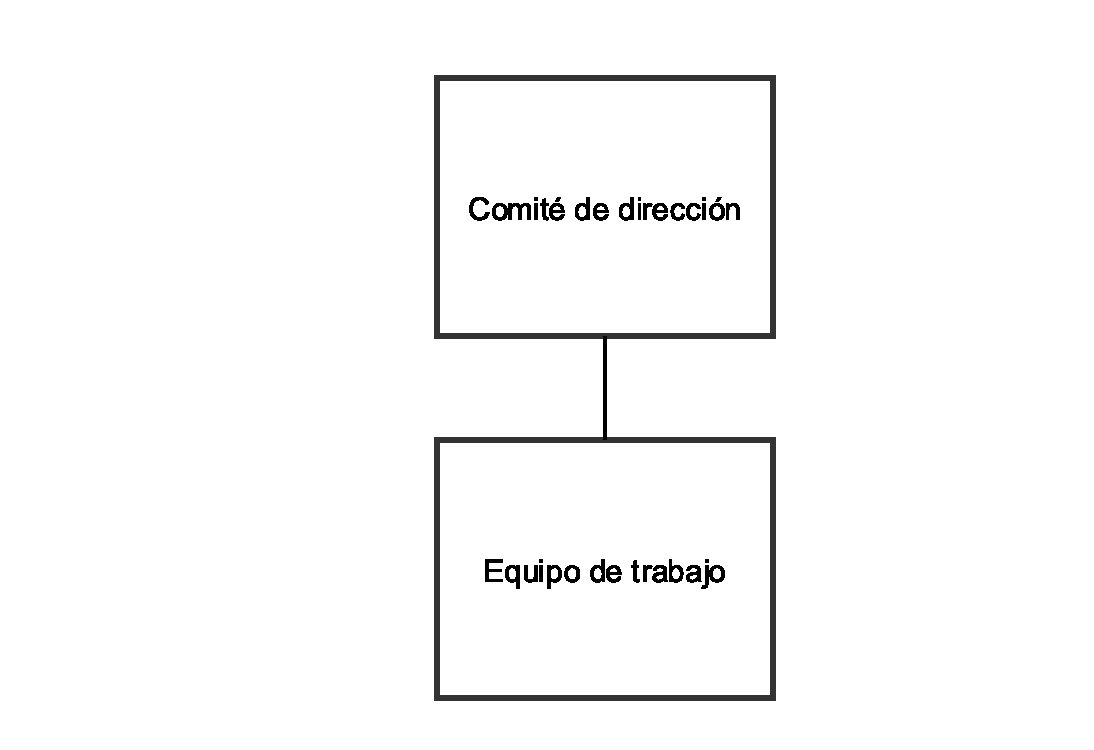
\includegraphics[scale=.75]{fig/organization}
	\caption{Esquema organizativo}
\end{figure}

\begin{itemize}
	\item Comité de dirección: su función principal es orientar por dónde debería ir el proyecto y tomar las decisiones finales a la hora de qué hacer o no.  Además, este comité deberá aprobar las diferentes fases del proyecto.
	\item Equipo de trabajo: el órgano encargado de diseñar y desarrollar el contenido del proyecto en función de las diferentes fases estipuladas.
\end{itemize}